

 \chapter{An enchanting mock chapter 1 title goes here} 

 \graphicspath{{mock_Chapter1/}} 

 


    \textbf{\emph{Abstract}}

    Important note about section headings:

In order to get both markdown (notebook) and latex playing ball, I: -
Use heading one in the notebook for Chapter number - Use heading two in
notebook for chapter title - Set chapter heading one block in nbconvert
template file to blank - \ldots{}result = heading ones are ommitted in
latex docs. Latex adds its own titles anyway (this is why I wanted to
sort this).

    Now: the question is - will things be excluded because they are in
markdown cells, of because of the nbconvert template.

Test:

\begin{itemize}
\item
  chapter sub title is current not in html tags and not blocked
\item
  \ldots{}but chapter number is in markdown
\item
  \ldots{}so: should be excluded in markdown
\end{itemize}

1: chapter 1 title and subtitle in heading 1, but chapter 1 number in
html 2 - chapter 1 in title and chapter 2 in subtitute - switch on
suppresion of chapter in nbconvert

    Lorem ipsum blah blah


    \section{Background}


    blah blah blah


    \section{Methods}


    blah blah blah

    \begin{figure}[htbp]
\centering
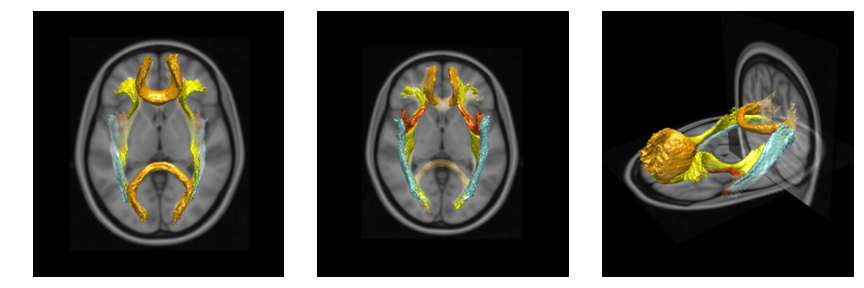
\includegraphics{figures/Ch2_JHU_tracts.png}
\caption{JHU tracts \{Adding a fuller caption which is what I woudl like
to say about the JHU tracts. Hopefuly this will not appear in the list
of figures. If the label tag does its job, I think that's what should
happen. But there's also this issue about closing the square
bracket\ldots{} \label{fig:JHU tracts}}
\end{figure}

HTML caption here - JHU tracts Adding a fuller caption which is what I
woudl like to say about the JHU tracts. Hopefuly this will not appear in
the list of figures. If the label tag does its job, I think that's what
should happen. But there's also this issue about closing the square
bracket\ldots{}

    blah blah blah


    \section{Results}


    blah blah blah

    \begin{figure}[htbp]
\centering
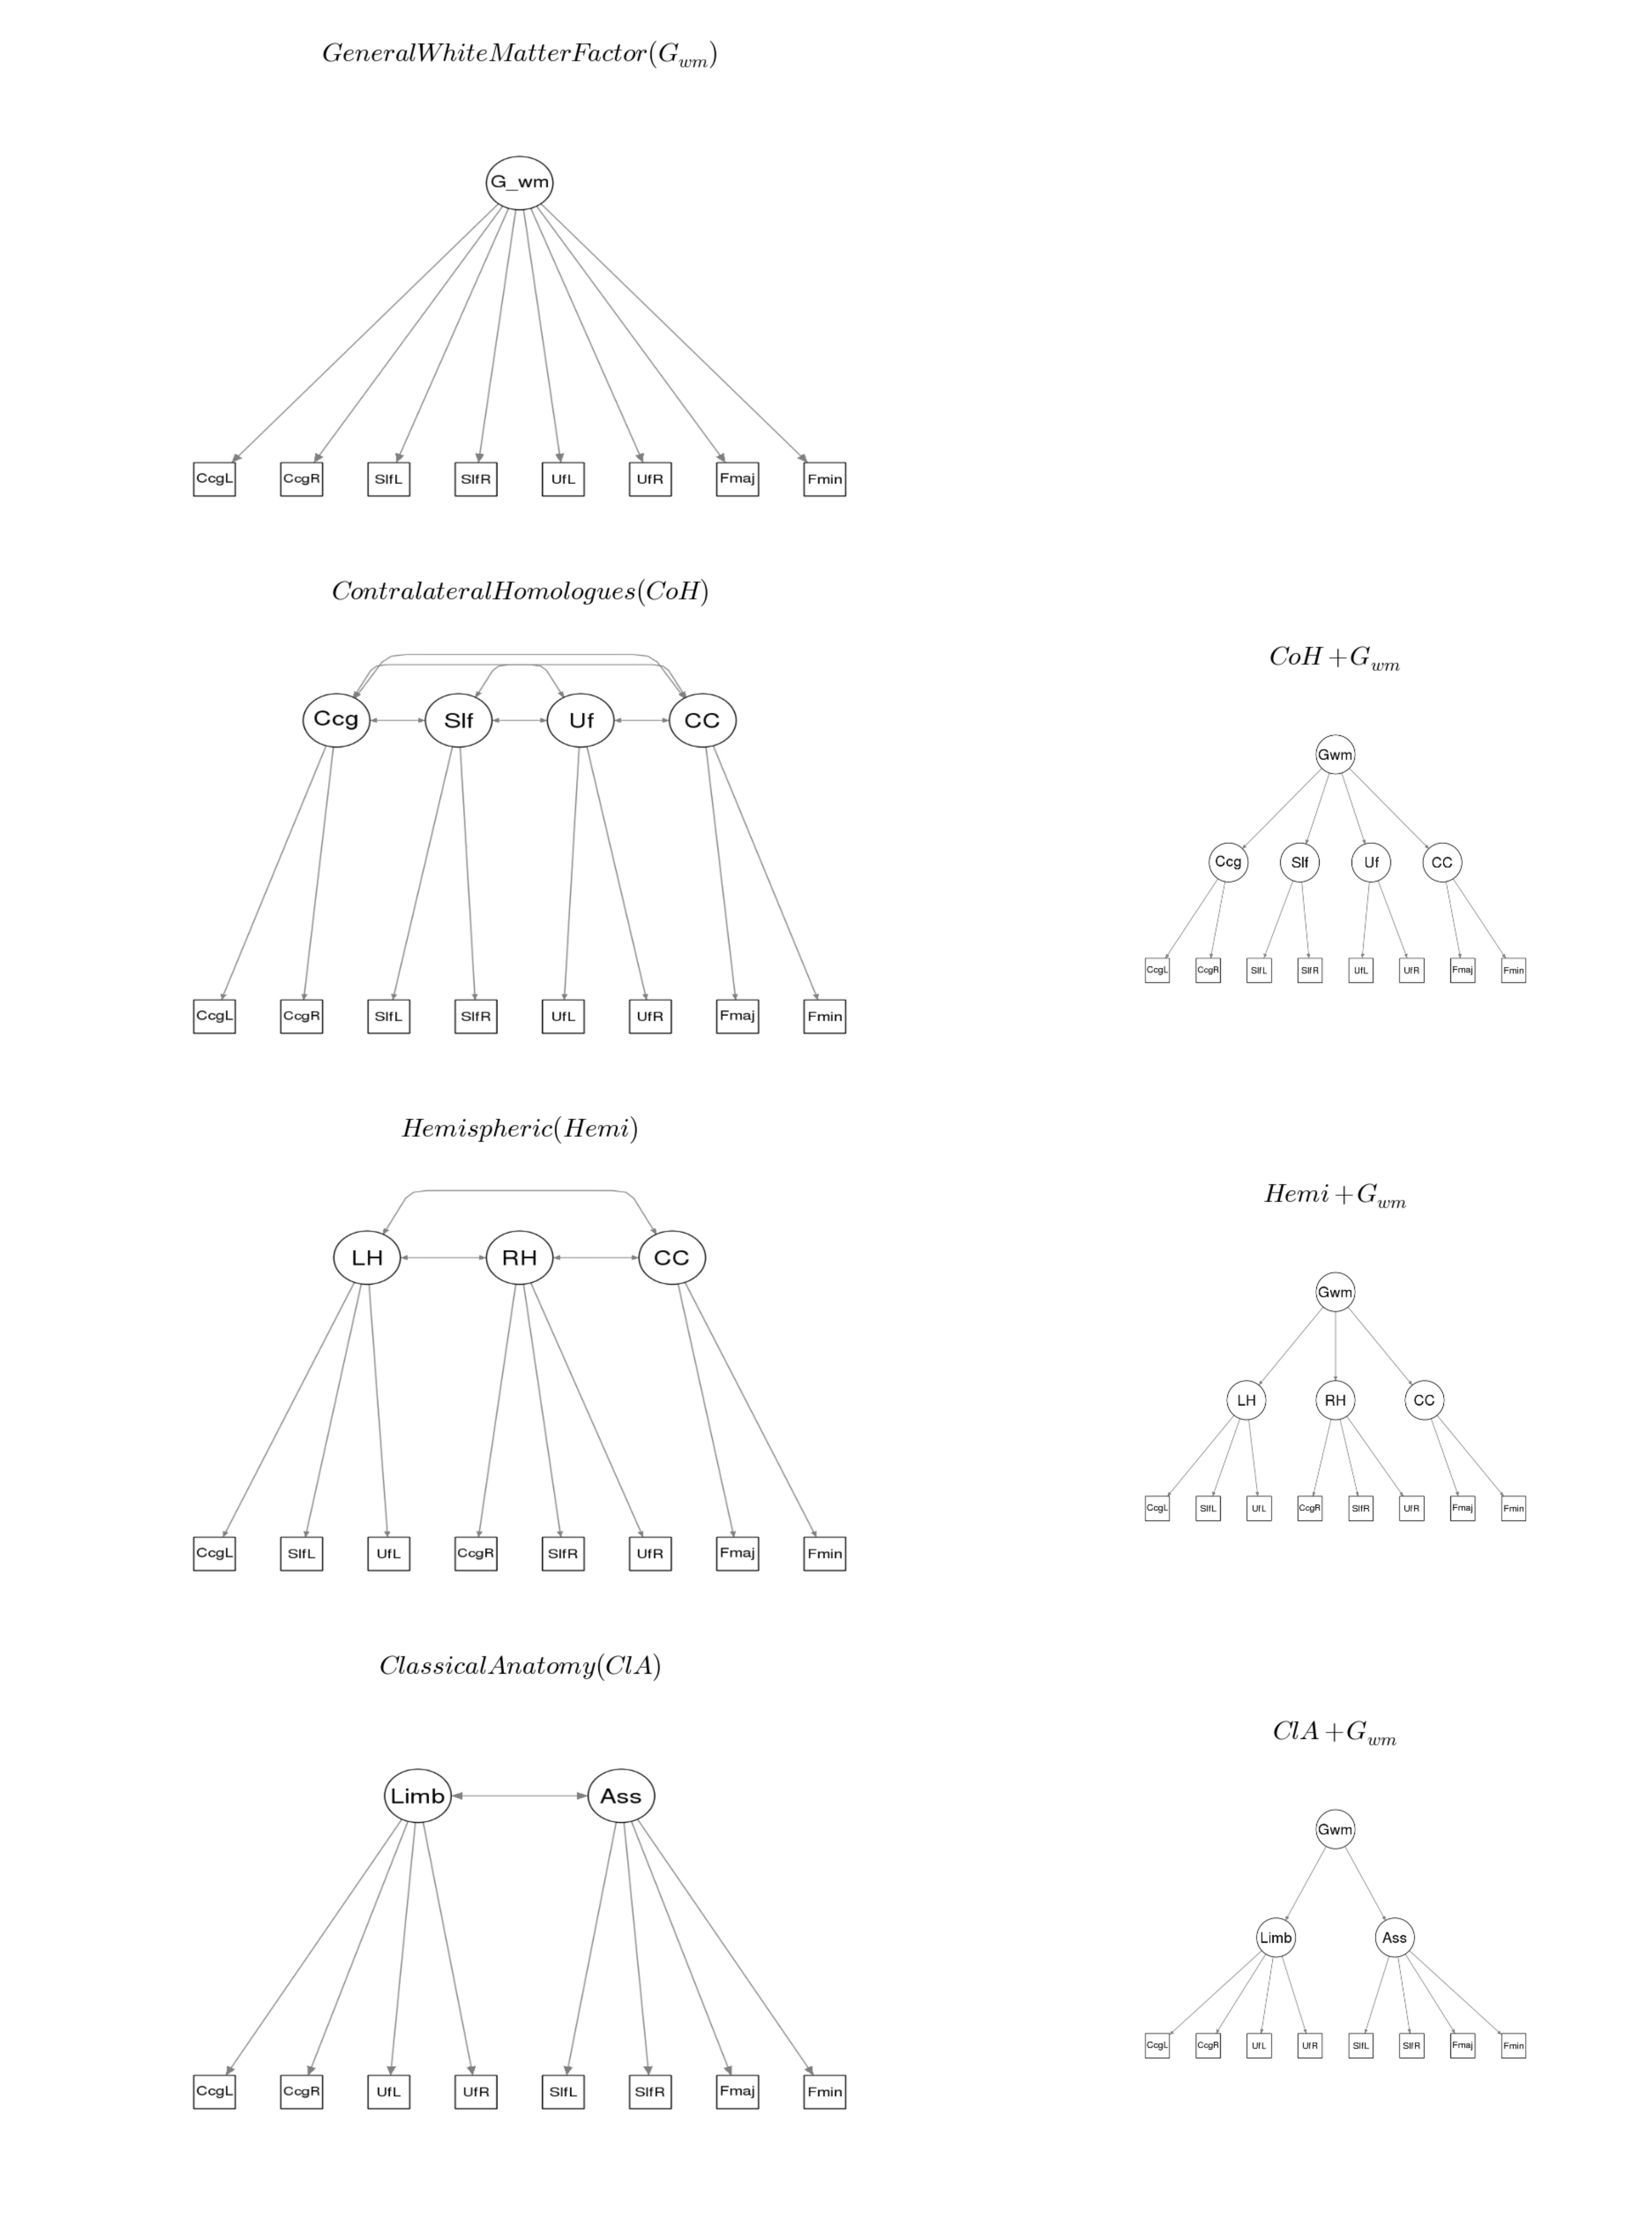
\includegraphics{figures/SEM_models.png}
\caption{SEM models \label{fig:SEM models}}
\end{figure}

HTML caption here - SEM models


    \section{Discussion}


    Minion hyperlink test

(see here
https://groups.google.com/forum/\#!msg/pandoc-discuss/MxGKvnNI08c/M6398LGWvqIJ)

    
\includegraphics{figures/minion.png}\{\#minion\}

HTML caption - minion (original pandoc hyperlink test)

    blah blah blah

    Alternative hyperlink test - see here:

\begin{verbatim}
http://stackoverflow.com/questions/9434536/how-do-i-make-a-reference-to-a-figure-in-markdown-using-pandoc
\end{verbatim}

    \begin{figure}[htbp]
\centering
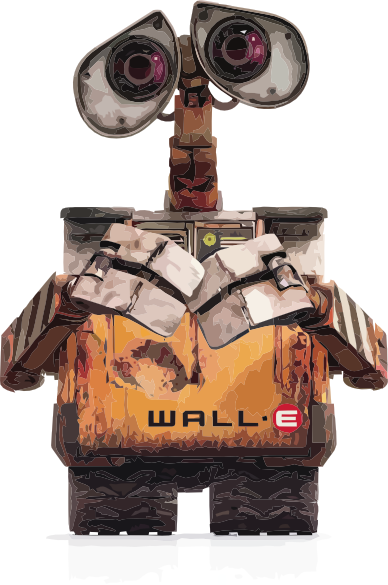
\includegraphics{figures/WallE.png}
\caption{WallE\label{fig:WallE}}
\end{figure}

Wall E HTML caption goes here; shouldn't be see by latex.

    blah blah blah

    \begin{figure}[htbp]
\centering

\includegraphics{figures/TomandJerry.png}
\caption{TomandJerry\label{fig:TomandJerry}}
\end{figure}

HTML caption here

    blah blah blah




    {Mock Chapter 2}



    